\section{Methods}

The \soft{HALFpipe} software is containerized, similar to \soft{fMRIPrep} or \soft{C-PAC}. This means that it comes bundled with all other software that is needed for it to run, such as \soft{fMRIPrep} \parencite{esteban2019a}, \soft{MRIQC} \parencite{esteban2017}, \soft{FSL} \parencite{jenkinson2012}, \soft{ANTs} \parencite{avants2011}, FreeSurfer \parencite{fischl2000}, and \soft{AFNI} \parencite{cox1996,cox1997}. As such, all users of one version of \soft{HALFpipe} will be using identical versions of these tools, because they are packaged with the container. Thus, the containerization of \soft{HALFpipe} software aids reproducibility across different researchers and computing environments.

We have provided the \soft{HALFpipe} application in a Singularity container and a Docker container. Singularity or Docker, which are both freely available, must be installed prior to downloading the containerized \soft{HALFpipe} application. Both Docker and Singularity perform so-called operating-system-level virtualization, but are more efficient and require less resources than virtual machines. Running Docker containers on a Linux or macOS operating system usually requires administrator privileges. Singularity is typically run on a Linux operating system, and may be used without administrator privileges. Docker can be run on the Windows operating system, but compatibility issues may occur with respect to file systems.

Our \soft{HALFpipe} development team adopted other software engineering best practices, which promoted faster development and reduced code errors. These industry best-practices, which have found their way into research applications \parencite{das2018}, involve writing code that is easy to read (albeit generally harder to write), the breakdown of complex systems into several simpler subsystems, dedicated effort toward thoughtful code design before implementation, and performing continuous integration via unit tests \parencite{beck2000}.

\subsection{Ecosystem}

\soft{HALFpipe} has been developed as an open-source project and is accepting contributions that offer new features, enhance functionality, or improve efficiency. All changes are tracked using the \soft{Git} version control system, which is the de-facto standard in the open source community. Additionally, before inclusion in the source tree, changes will be reviewed and then undergo automated testing, which includes unit tests and also running an entire analysis for one subject of the OpenNeuro dataset ds000108 \parencite{wager2008}. This way unexpected side effects and bugs will be caught and corrected before causing problems for users.

\soft{HALFpipe} releases are made using semantic versioning as adapted for compatibility with Python \parencite{coghlan2013}. This means that there will be feature releases that add new functionality and patch releases that make minor adjustments to solve specific issues or bugs. The development team takes great care that new patch releases of dependencies such as \soft{fMRIPrep} are regularly incorporated into \soft{HALFpipe} so that bug fixes are made available to users.

\soft{HALFpipe} currently depends on the long-term support release 20.2.x of \soft{fMRIPrep}. For future releases containing new features, the developers will approve  possible upgrades that are advantageous to ENIGMA consortium projects. We may also consider replacing tools used for specific processing steps or upgrading the standard brain template in future releases based on such considerations, which will be explained in the change log of each release.


\subsection{Databases}

To automatically construct a neuroimaging data processing workflow, the program needs to be able to fulfill queries such as \pseudocode{``retrieve the structural image for subject x''}. Many programs implement such queries using a database system. The queries also need to flexibly interface with the logic of neuroimaging and processing pipelines, which is relevant in the context of missing scans.

In the context of missing scans, \soft{HALFpipe} always tries to execute the best possible processing pipeline based on the data that is available. For example, a field map may have been routinely acquired before each functional scan in a particular dataset. If one of these field maps is missing, \soft{HALFpipe} flexibly assigns another field map, for example one belonging to the preceding functional scan. However, \soft{HALFpipe} will not use a field map from another scan session, as field inhomogeneities are likely to have changed. Finally, \soft{HALFpipe} does not fail if a field map is missing, but simply omits the distortion correction step for that subject. Other examples include the ability of \soft{HALFpipe} to match structural to functional images, and match task events to a functional scan. This strategy is used throughout the construction of processing workflows.


\subsection{Metadata}

Processing of neuroimaging data requires access to relevant metadata, such as temporal resolution, spatial resolution, and many others. Some elements of metadata, such as echo time (TE), are represented differently depending on scanner manufacturer and DICOM conversion software. The method for reading various types of data has been harmonized in \soft{HALFpipe} using the following three methods.

First, metadata can be stored in BIDS format. This means that a JavaScript Object Notation (JSON) file accompanies each image file, which contains the necessary metadata. BIDS calls this file the \term{sidecar}, and common tools such as \soft{heudiconv} \parencite{halchenko2018} or \soft{dcm2niix} \parencite{li2016} generate these files automatically. If these files are present, \soft{HALFpipe} will detect and use them. Second, instead of sidecar files, some software tools store image metadata in the NIfTI header. The NIfTI format defines fields that can fit metadata, but depending on how the image file was created, these metadata may be missing. Some conversion programs also place the metadata in the description field in free text format. This description can also be parsed and read automatically. Third, information may be incorrectly represented due to user error, incompatible units of measurement, or archaic technical considerations. In such cases, \soft{HALFpipe} provides a mechanism to override the incorrect values. For every metadata field, the user interface will prompt the user to confirm that metadata values have been read or inferred correctly. The user can choose to manually enter the correct values.


\subsection{Interfaces}

\soft{HALFpipe} consists of different modules that need to pass data between each other, such as file pathnames and the results of quality assessment procedures. Developing an application as large and complex as \soft{HALFpipe} requires establishing predictable interfaces, which prescribe data formats for communication within the application. An advantage of this approach is that knowledgeable users can write their own code to interface with \soft{HALFpipe}.

\soft{HALFpipe} uses the Python module \soft{marshmallow} to implement interfaces, called schemas in the module's nomenclature. All schemas are defined in the \code{halfpipe.schema} module. When the user first starts the application, the user interface is displayed by \soft{HALFpipe}. It asks the user a series of questions about the data set and the analysis plan, and stores the inputs in a configuration file called \filename{spec.json}. The configuration file has predictable syntax and can be easily scripted or modified, which enables collaborative studies to harmonize analysis plans.


\subsection{Workflow engine}

To obtain reproducible results, a core requirement for \soft{HALFpipe} was reproducible execution of the processing pipeline. As the ENIGMA consortium requires fMRI analysis of large datasets with several thousand samples, \soft{HALFpipe} was designed to parallelize processing on multiple computers or processor cores. Both of these specifications were achieved by implementation in \soft{Nipype}, \term{NeuroImaging in Python: Pipelines and Interfaces} \parencite{gorgolewski2011}. \soft{Nipype} is a workflow engine for neuroimaging that constructs an acyclic directed graph, in which nodes represent processing commands that need to be executed (the steps of the pipeline), while the edges represent inputs and outputs being passed between nodes (images or text files). In this formalization of a neuroimaging pipeline as a graph, the fastest order for execution across multiple processor cores can be determined.

The workflow graphs are modular and scalable, which means they can be nested and extended. \soft{HALFpipe} uses the workflows defined by \soft{fMRIPrep} and then connects these outputs to additional workflows. \soft{fMRIPrep} itself is modular and divided into multiple workflows: \soft{sMRIPrep} \parencite{esteban2021b}, \soft{SDCFlows} \parencite{esteban2020a}, \soft{NiWorkflows} \parencite{esteban2021a}, and \soft{NiTransforms} \parencite{goncalves2021}. The workflow graph facilitates saving and verifying intermediate results, and supports the user's ability to stop and later restart processing. \soft{HALFpipe} also uses the graphs to determine which intermediate results files are not needed by subsequent commands by using a tracing garbage collection algorithm \parencite{dijkstra1978}. As such, intermediate files do not accumulate on the storage device. This feature is implemented as a plugin to \soft{Nipype}.

\soft{Nipype} forms the basis of \soft{fMRIPrep} and \soft{C-PAC}, which are widely used in the neuroimaging community. However, it has several limitations that are relevant in the context of \soft{HALFpipe}. \soft{HALFpipe} is able to calculate features and statistical maps with different variations of preprocessing settings. To do this efficiently, intermediate results need to be re-used whenever possible. An improved second version of \soft{Nipype} is currently being developed, called \soft{Pydra} \parencite{jarecka2020}, which will be able to automatically detect repetitive processing commands, and automatically re-use outputs. Presently, until \soft{Pydra} becomes available, \soft{HALFpipe} calculates a four-letter hash code that uniquely identifies each pre-processing step. Before constructing a new pre-processing command, \soft{HALFpipe} checks whether its hash has already been added to the graph. If present, the existing command is re-used, significantly reducing processing times in the context of multiverse analysis or pipeline comparison (see Table~\ref{table:runtimes}).

\begin{tablebox}[label={table:runtimes}]{Efficient pipeline construction speeds up multiverse analyses}

A core feature of \soft{HALFpipe} is the ability to explore the impact of different preprocessing strategies on results. For a face matching task data set \parencite{wakeman2015}, participant \emph{01} was entered into \soft{HALFpipe} and task contrasts were calculated with three pipelines.

First we used the recommended settings from Table~\ref{table:settings}. For the second and third pipelines we used the same settings but disabled \soft{ICA-AROMA}. For the second pipeline we additionally added the motion parameters to the task model as confound time series. The third pipeline did not include any denoising or confound time series removal.

The naive approach is to run \soft{HALFpipe} three times, once for each pipeline. This approach is sub-optimal, as many duplicate computations are performed. By default, \soft{HALFpipe} combines all three pipelines and executes them so that no duplicate computations are performed, making processing much faster. Processing was done on an \emph{AMD Ryzen Threadripper 2950X} 16-core processor, and each run of \soft{HALFpipe} was configured to use all cores. The table shows the processing time (\emph{wall clock time}) spent on each pipeline. For the naive approach, we also show the total time.
\\

\begingroup%
\fboxsep=1pt%
\newcolumntype{L}{>{\raggedright\arraybackslash}X}%
\newcolumntype{K}[1]{>{\raggedright\arraybackslash}m{#1}}%
\renewcommand{\arraystretch}{1.35}%
\begin{tabularx}{\textwidth}{@{} | K{2cm} |
L | L | @{}}
\hhline{~|-|-|}
\multicolumn{1}{c|}{} &
\textbf{Naive approach} &
\textbf{Combined approach (via hashing algorithm)} \\
\hhline{-|-|-|}
Processing time (hh:mm) &%
01:39 + 01:36 + 01:33 = \textbf{04:49} &%
\textbf{01:43} \\
\hhline{-|-|-|}
\end{tabularx}\par
\endgroup

\end{tablebox}


A key requirement of \soft{HALFpipe} was robust and flexible handling of missing data. For instance a missing functional scan or statistical map does not cause \soft{HALFpipe} to fail. Additionally, \soft{HALFpipe} defines inclusion and exclusion criteria for scans, such as the maximum allowed motion (mean framewise displacement) or a minimum brain coverage when extracting a brain region's average signal. Finally, depending on the data set, statistical maps may need to be aggregated across runs or sessions within single subjects before a group-level model can be run. This means that the static graph has to be modified dynamically to adapt to the results of processing. \soft{HALFpipe} solves this problem by defining a data structure that not only contains the file names of statistical maps, but also the tags and metadata that can be used to adjust processing on the fly. For example, using this data structure, design matrices can be constructed for group models based on the actual subjects that have statistical maps available.


\subsection{Preprocessing}\label{sec:preprocessing}

Main preprocessing is done in \soft{HALFpipe} with \soft{fMRIPrep}, which performs a consensus of preprocessing steps required for any fMRI study \parencite{esteban2019a}. Consensus steps for structural images include skull stripping, tissue segmentation, and spatial normalization. Consensus steps for functional images include motion correction, slice time correction, susceptibility distortion correction, coregistration, and spatial normalization (Figure~\ref{fig:workflow}).

\soft{HALFpipe} defines standard space as the \term{MNI152NLin2009cAsym} template, which is the most current and detailed template available (Horn 2016a). Note that the standard space template is not user-configurable, so that any outputs generated by one version of \soft{HALFpipe} can be easily compared to outputs generated by another version of \soft{HALFpipe}.

Once the fMRI data have been processed with \soft{fMRIPrep} and resampled into standard space, \soft{HALFpipe} implements a number of additional preprocessing steps for denoising, filtering, and harmonizing the functional data (see also Figure~\ref{fig:workflow}):

\begin{enumerate}[leftmargin=*]

\item

\soft{ICA-AROMA} is an algorithm based on independent component analysis. It classifies components into those that contain signal and those that are noise \parencite{pruim2015}. To accomplish this, \soft{ICA-AROMA} relies on reference templates defined in \term{MNI152NLin6Asym} space, which is different from the standard space template \term{MNI152NLin2009cAsym} that is used by \soft{fMRIPrep}. To allow \soft{ICA-AROMA} to run, it is thus necessary to provide the preprocessed image not just in the default template space, but also in the one required by \soft{ICA-AROMA}. By default, \soft{fMRIPrep} will estimate a second normalization to this other template, apply it to the fMRI image in native space, and run \soft{ICA-AROMA} on the resulting image \parencite{ciric2021}. This approach effectively doubles the processor time spent on spatial normalization, and may require manually checking both spatial registrations.

To avoid this considerable effort, \soft{HALFpipe} implements a different approach by using an existing warp between the two standard template spaces \parencite{horn2016c}. This predefined warp is concatenated with the normalization that was already estimated by \soft{fMRIPrep}, and then a second round of resampling is performed with \soft{fMRIPrep}'s \code{bold\_std\_trans\_wf} This way, only the resampling step needs to be run twice.

Finally, \soft{ICA-AROMA} is run on the resulting fMRI image in \term{MNI152NLin6Asym} space using \soft{fMRIPrep}'s \code{ica\_aroma\_wf} workflow, which also includes spatial smoothing fixed to a 6 mm FWHM smoothing kernel. The resulting classifications are kept for step~\ref{itm:aroma}.

\item

\soft{HALFpipe} implements spatial smoothing using \soft{AFNI}'s \soft{3dBlurToFWHM} \parencite{friedman2006}. Each voxel's signal is averaged with the signal of surrounding voxels weighted by an isotropic gaussian kernel. At the edges of the brain, this kernel may include non-brain voxels, so smoothing is constrained by the brain mask. This is equivalent to the procedure in the \term{Minimal Preprocessing Pipelines for the Human Connectome Project} \parencite{glasser2013}. In addition, \soft{3dBlurToFWHM} estimates the smoothness of the resulting image, and iteratively decreases the amount of smoothing so that the resulting smoothness matches the user setting. This way, differences in the intrinsic smoothness between datasets (e.g., due to different voxel sizes) can be harmonized.

\item\label{itm:grandmean}

Grand mean scaling sets the image mean, defined as the within-scan mean across all voxels and time points, to a predefined value. The grand mean is closely related to scanner parameters such as RF power or amplifier gain but not to neural mechanisms \parencite{gavrilescu2002}. Adjusting the grand mean via scaling makes analysis results more interpretable and comparable across subjects, sessions, and sites. The scaling factor is calculated based on the masked functional image, and applied to both the fMRI data and the confound time series extracted by \soft{fMRIPrep}.

\item\label{itm:aroma}

If selected, the previously estimated \soft{ICA-AROMA} noise components are removed from the smoothed and grand-mean-scaled fMRI data. This is done in a non-aggressive way to minimize removing variance that is shared between signal and noise components. \soft{ICA-AROMA} implements this step using the \soft{FSL} command \soft{fsl\_regfilt}, which calculates an ordinary least squares regression for each voxel, where the design matrix includes both the signal and the noise components as regressors. This means that the resulting regression weights reflect the unique variance of the noise components (and not the shared variance with signal components). Then, the noise component regressors are multiplied by their regression weights and these products are added together to yield one time series of the noise. Subtracting the noise from the voxel time series yields a denoised time series (the regression residuals). This step is done using a custom re-implementation of \soft{fsl\_regfilt} in \soft{HALFpipe} using \soft{Numpy} \parencite{harris2020}.

\item\label{itm:tempfilt}

Temporal filtering can be selected to remove low-frequency drift via a high-pass filter, high-frequency noise via a low-pass filter, or both at the same time using a band-pass filter. \soft{HALFpipe} implements two approaches to temporal filtering, a frequency-based approach \parencite{jo2013} and a Gaussian-weighted approach \parencite{marchini2000}. The frequency-based temporal filter is very exact in selecting frequencies to be kept or removed, and is commonly used to calculate fractional Amplitude of Low Frequency Fluctuations (fALFF) and Regional Homogeneity (ReHo). The Gaussian-weighted temporal filter is the default used by \soft{FSL Feat} \parencite{jenkinson2012} and may have fewer edge effects at the start and end of the time series. However, its spectrum also has a more gradual roll-off, meaning that it will be less aggressive in removing frequencies close to the chosen cutoff value.

\end{enumerate}

Importantly, \soft{HALFpipe} runs \soft{fMRIPrep} with small modifications. For instance, we disabled \soft{fMRIPrep}’s experimental susceptibility distortion correction in the absence of field maps, because it is not yet validated. Further, \soft{HALFpipe} suggests default settings for each preprocessing step, which are outlined in Table~\ref{table:settings}. Note that some are selected based on best-practices in the field (i.e., band-pass temporal filter for ALFF and ReHo), whereas most default settings can be adjusted by the user. Last, \soft{HALFpipe} does not output preprocessed and normalized functional images by default, because they use a lot of disk space. However, in the user interface users can manually choose to output a preprocessed functional image with their choice of preprocessing settings.

\begin{figure}[!tb]
    \begin{adjustwidth}{-1cm}{}
        \hsize=\linewidth%
        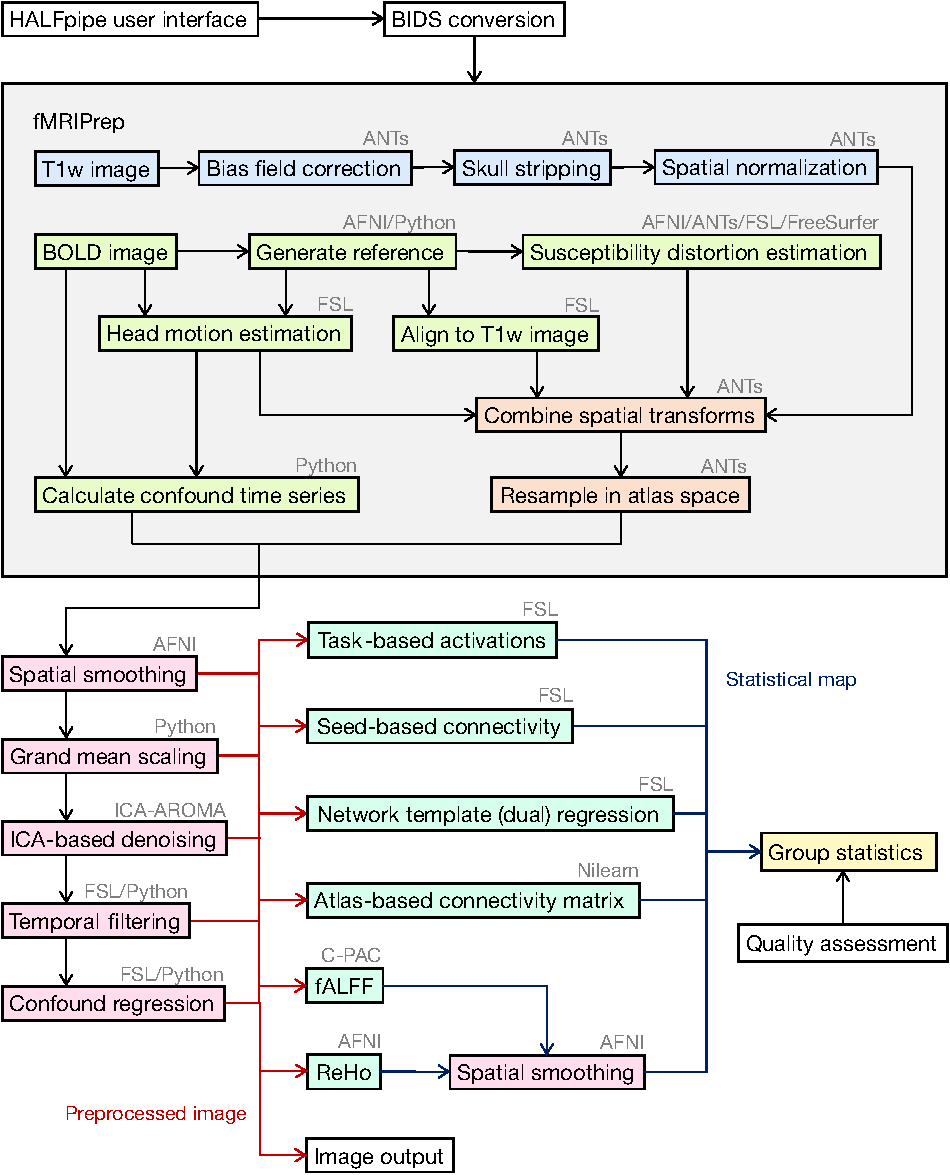
\includegraphics[width=\linewidth]{fig/workflow/workflow-crop}
        \caption{\textbf{\soft{HALFpipe} workflow.} \soft{HALFpipe} is configured in a user interface where the user is asked a series of questions about their data and the processing steps to perform. Data is then converted to BIDS format \parencite{gorgolewski2016b} to allow standardized processing (white). After minimal preprocessing of the structural (blue) and functional (green and orange) data with \soft{fMRIPrep} \parencite{esteban2019a}, additional preprocessing steps can be selected (red). Using the preprocessed data, statistical maps can be calculated during feature extraction (turquoise). Finally, group statistics can be performed (yellow). Note that not all preprocessing steps are available for each feature, as is outlined in Table~\ref{table:settings}. The diagram omits this information to increase visual clarity.}\label{fig:workflow}
  \end{adjustwidth}
\end{figure}


\subsection{Confound time series removal}

fMRIprep not only outputs a preprocessed image in standard space but also a spreadsheet with confound time series named confounds.tsv. These include the (derivatives of) motion parameters (squared), aCompCor components (Behzadi et al. 2007), white matter signal, CSF signal, and global signal (Figure 3). A key consideration needs to be made when using fMRIPrep confound time series in conjunction with the preprocessing steps outlined in the previous section: Using confound time series as nuisance regressors with data that was temporally filtered or denoised can re-introduce the removed temporal or noise signals back into the voxel time series (Hallquist, Hwang, and Luna 2013).

An example of this phenomenon may be regressing out a set of fMRIPrep confound time series after removing low-frequency drift via temporal filtering. In practice, this means setting up a regression model for each voxel, where the voxel time series is the dependent variable and the regressors are the confound time series. The regression will yield a weight for each confound time series, so that the total model explains the maximum amount of variance (under assumption of normality). After multiplying the confound time series with these weights, their products are summed to one time series containing the confound-related signal in that voxel. This time series is then subtracted from the original voxel time series to get the result (i.e., the regression residuals). However, if the confound time series happen to contain any low-frequency drift, then their weighted sum likely will as well. It follows that subtracting a time series with temporal drift from the temporally filtered voxel data will re-introduce temporal drift, independent of whether a temporal filter was applied before.

In HALFpipe, any (optional) denoising or filter applied to the voxel time series is also applied to the fMRIPrep confound time series. This way, previously removed variance is not re-introduced accidentally, because it has been removed from both sides of the regression equation. For example, when the user chooses to perform ICA-AROMA denoising, then the same denoising will be applied to the time fMRIPrep confound time series, and the same applies when using a temporal filter. Note that this means that the confound time series generated by HALFpipe will be different from the original fMRIPrep confound time series, and users should take care to use the appropriate file when running custom analyses.


\subsection{Quality assessment}\label{sec:qamethods}

Assessing the quality of data and preprocessing is a laborious undertaking and often done manually. Efforts to automate this process, either through predefined thresholds of image quality features \parencite{alfaroalmagro2018} or machine learning \parencite{esteban2017} are not yet ready to replace the eyes of a trained researcher checking the data. However, various approaches make this process easier. First, rather than viewing three-dimensional neuroimaging files directly, generating and viewing reports containing two-dimensional images offers a significant time savings. Second, tools such as \soft{slicesdir} (in \soft{FSL}), \soft{fMRIPrep}, and \soft{MRIQC} generate HTML files that contain multiple report images and can be explored in a web browser. \soft{MRIQC} also provides an interactive widget to rate the quality of each image \parencite{esteban2019b}.

In \soft{HALFpipe}, we use a fixed set of processing steps for quality assessment. While \soft{slicesdir} allows the researcher to easily compare the same image type across different subjects, it cannot be used to generate reports for all types of images. By contrast, \soft{fMRIPrep}/\soft{MRIQC} HTML files have a broad range of information and quality report images included, but one HTML file is always specific to one subject. As such, examining multiple processing steps in many subjects can be cumbersome.

To overcome these issues, \soft{HALFpipe} provides an interactive web app that is contained in a single HTML file. The app dynamically loads reports with images, and can handle datasets up to thousands of images without a performance penalty. The images can be sorted both by subject, as is done by \soft{fMRIPrep}/\soft{MRIQC}, or by image type, as is done in \soft{slicesdir}. Each image can be rated as either good, uncertain, or bad. Predefined logic automatically converts these ratings into inclusion/exclusion decisions for \soft{HALFpipe}'s group statistics. In addition, tagging images as uncertain enables users to efficiently retrieve and discuss these with a colleague or collaborator, after which a definitive decision on image quality can be made.


\subsection{Group statistics}\label{sec:statistics}

\soft{HALFpipe} uses \soft{FSL} FMRIB Local Analysis of Mixed Effects \parencite[FLAME,][]{woolrich2004} for group statistics, because FLAME considers the within-subject variance of lower level estimates in its mixed effects models. In addition, its estimates are conservative, which means they offer robust control of the false positive rate \parencite{eklund2016}.

A common issue in fMRI studies is that the spatial extent of brain coverage may differ between subjects. A common choice is to restrict higher-level statistics to only those voxels that were acquired in every subject. However, with a large variation in brain coverage, which is to be expected when pooling multi-cohort data, sizable portions of the brain may ultimately be excluded from analysis. To circumvent this issue, \soft{HALFpipe} uses a re-implementation of FLAME in \soft{Numpy} \parencite{harris2020}. In this implementation, a unique design matrix is generated for every voxel so that only subjects who have a measurable value for a given voxel are included. Then the model is estimated using the FLAME algorithm. This list-wise deletion approach depends on the assumption that voxels are missing completely at random (MCAR), meaning that the regressors (and thus statistical values) are independent of scanner coverage.

For group models, users can specify flexible factorial models that include covariates and group comparisons. By default, missing values for these variables are handled by list-wise deletion as well, but the user may alternatively choose to replace missing values by zero in the demeaned design matrix. The latter approach is equivalent to imputation by the sample mean. Design matrices for the flexible factorial models are generated using the Python module \soft{Patsy} \parencite{smith2018}. Contrasts between groups are specified using the \soft{lsmeans} procedure \parencite{lenth2016}.


\subsection{Running on a high-performance cluster}\label{sec:runningonhpc}

Deploying \soft{Nipype} to perform computations on multiple nodes, such as on a high performance cluster (HPC) is particularly challenging. By default, \soft{Nipype} submits a separate job to the cluster queue for each processing command (graph node) regardless of the amount of time required to execute the command. A watcher process running on the head node collects outputs from completed commands and submits the next processing command. This process can be inefficient on some HPCs because computational resources need to be allocated and deallocated continually. We implemented a more efficient approach for \soft{HALFpipe} that partitions the processing graph into many independent subgraphs, which the user may submit as separate jobs. The smallest granularity available is one subgraph per subject that is invoked automatically with the command line flag \code{--use-cluster}. A \soft{Nipype} workflow is created and validated for all subjects before the pipeline starts running. In a cluster setting, the most efficient resource utilization is to submit each subject as a separate job and to run each job on two CPU cores.


\begin{tablebox}[label={table:settings}]{Default values for preprocessing settings per feature}

\begingroup%
\newcolumntype{L}{>{\raggedright\arraybackslash}X}%
\newcolumntype{C}{>{\centering\arraybackslash}X}%
\newcolumntype{K}[1]{>{\raggedright\arraybackslash}m{#1}}%
\newcolumntype{M}[1]{>{\centering\arraybackslash}m{#1}}%
\renewcommand\tabularxcolumn[1]{m{#1}}%
\renewcommand{\arraystretch}{1.35}%
\begin{tabularx}{\textwidth}{@{} | K{2cm} |
M{1.9cm} | C | C | M{1.4cm} | C | c | c | @{}} 
\hhline{~|-|-|-|-|-|-|-|}
\multicolumn{1}{c|}{} & 
\textbf{Preprocessed image} & 
\textbf{Task-based activation} &
\textbf{Seed-based connectivity} & 
\textbf{Dual regression} &
\textbf{Atlas-based connectivity matrix} & 
\textbf{ReHo} & 
\textbf{fALFF} \\
\hhline{-|-|-|-|-|-|-|-|}
Spatial smoothing &%
\multicolumn{4}{c|}{\cellcolor{leaLightGreen}6 mm} &%
\cellcolor{leaGrey} &%
\multicolumn{2}{c|}{\cellcolor{leaLightGreen}6 mm*} \\
\hhline{-|-|-|-|-|-|-|-|}
Grand mean scaling &%
\multicolumn{7}{c|}{\cellcolor{leaLightGreen}10,000} \\
\hhline{-|-|-|-|-|-|-|-|}
ICA-AROMA &%
\multicolumn{7}{c|}{\cellcolor{leaLightGreen}Yes} \\ [2ex]
\hhline{-|-|-|-|-|-|-|-|}
Temporal filter &%
\multicolumn{4}{c|}{\cellcolor{leaLightGreen}Gaussian (128 s FWHM)} &% 
  \multicolumn{3}{c|}{\cellcolor{leaLightGreen}Frequency-based (0.01--0.1 Hz)} \\ [2ex]
\hhline{-|-|-|-|-|-|-|-|}
Confound removal &%
\cellcolor{leaLightGreen}None &%
\multicolumn{3}{c|}{\cellcolor{leaGrey}} &%
\multicolumn{3}{c|}{\cellcolor{leaLightGreen}None} \\
\hhline{-|-|-|-|-|-|-|-|}
Add confounds to model &%
\cellcolor{leaGrey}&%
\multicolumn{3}{c|}{\cellcolor{leaLightGreen}None} &%
\multicolumn{3}{c|}{\cellcolor{leaGrey}} \\
\hhline{-|-|-|-|-|-|-|-|}
\end{tabularx}\par
\vspace*{2mm}
Note: Cells filled in grey indicate that this option cannot be selected in
the user interface, all other settings can be adapted by the user; * done
on the statistical maps after feature extraction.
\endgroup

\end{tablebox}

